\documentclass{article}
\usepackage{graphicx} % for includegraphics
\usepackage{epsf} % for epsffile and epsfxsize

\begin{document}

This is an example tex file to show how to include a gnuplot generated
tex figure in your \LaTeX document. The following is the gnuplot
script used to generate the command. The output is in Fig.~\ref{fig1}:

\begin{verbatim}
set term latex
set size 1,1
set out 'gplt.tex'
set xlabel '$\theta$'
set ylabel '$sin(\theta)$'
plot sin(x) notitle
\end{verbatim}

\begin{figure}
% GNUPLOT: LaTeX picture
\setlength{\unitlength}{0.240900pt}
\ifx\plotpoint\undefined\newsavebox{\plotpoint}\fi
\sbox{\plotpoint}{\rule[-0.200pt]{0.400pt}{0.400pt}}%
\begin{picture}(1500,900)(0,0)
\sbox{\plotpoint}{\rule[-0.200pt]{0.400pt}{0.400pt}}%
\put(171.0,172.0){\rule[-0.200pt]{305.461pt}{0.400pt}}
\put(171.0,172.0){\rule[-0.200pt]{4.818pt}{0.400pt}}
\put(151,172){\makebox(0,0)[r]{-1}}
\put(1419.0,172.0){\rule[-0.200pt]{4.818pt}{0.400pt}}
\put(171.0,232.0){\rule[-0.200pt]{305.461pt}{0.400pt}}
\put(171.0,232.0){\rule[-0.200pt]{4.818pt}{0.400pt}}
\put(151,232){\makebox(0,0)[r]{-0.8}}
\put(1419.0,232.0){\rule[-0.200pt]{4.818pt}{0.400pt}}
\put(171.0,293.0){\rule[-0.200pt]{305.461pt}{0.400pt}}
\put(171.0,293.0){\rule[-0.200pt]{4.818pt}{0.400pt}}
\put(151,293){\makebox(0,0)[r]{-0.6}}
\put(1419.0,293.0){\rule[-0.200pt]{4.818pt}{0.400pt}}
\put(171.0,353.0){\rule[-0.200pt]{305.461pt}{0.400pt}}
\put(171.0,353.0){\rule[-0.200pt]{4.818pt}{0.400pt}}
\put(151,353){\makebox(0,0)[r]{-0.4}}
\put(1419.0,353.0){\rule[-0.200pt]{4.818pt}{0.400pt}}
\put(171.0,414.0){\rule[-0.200pt]{305.461pt}{0.400pt}}
\put(171.0,414.0){\rule[-0.200pt]{4.818pt}{0.400pt}}
\put(151,414){\makebox(0,0)[r]{-0.2}}
\put(1419.0,414.0){\rule[-0.200pt]{4.818pt}{0.400pt}}
\put(171.0,474.0){\rule[-0.200pt]{305.461pt}{0.400pt}}
\put(171.0,474.0){\rule[-0.200pt]{4.818pt}{0.400pt}}
\put(151,474){\makebox(0,0)[r]{ 0}}
\put(1419.0,474.0){\rule[-0.200pt]{4.818pt}{0.400pt}}
\put(171.0,534.0){\rule[-0.200pt]{305.461pt}{0.400pt}}
\put(171.0,534.0){\rule[-0.200pt]{4.818pt}{0.400pt}}
\put(151,534){\makebox(0,0)[r]{ 0.2}}
\put(1419.0,534.0){\rule[-0.200pt]{4.818pt}{0.400pt}}
\put(171.0,595.0){\rule[-0.200pt]{305.461pt}{0.400pt}}
\put(171.0,595.0){\rule[-0.200pt]{4.818pt}{0.400pt}}
\put(151,595){\makebox(0,0)[r]{ 0.4}}
\put(1419.0,595.0){\rule[-0.200pt]{4.818pt}{0.400pt}}
\put(171.0,655.0){\rule[-0.200pt]{228.373pt}{0.400pt}}
\put(1419.0,655.0){\rule[-0.200pt]{4.818pt}{0.400pt}}
\put(171.0,655.0){\rule[-0.200pt]{4.818pt}{0.400pt}}
\put(151,655){\makebox(0,0)[r]{ 0.6}}
\put(1419.0,655.0){\rule[-0.200pt]{4.818pt}{0.400pt}}
\put(171.0,716.0){\rule[-0.200pt]{228.373pt}{0.400pt}}
\put(1419.0,716.0){\rule[-0.200pt]{4.818pt}{0.400pt}}
\put(171.0,716.0){\rule[-0.200pt]{4.818pt}{0.400pt}}
\put(151,716){\makebox(0,0)[r]{ 0.8}}
\put(1419.0,716.0){\rule[-0.200pt]{4.818pt}{0.400pt}}
\put(171.0,776.0){\rule[-0.200pt]{305.461pt}{0.400pt}}
\put(171.0,776.0){\rule[-0.200pt]{4.818pt}{0.400pt}}
\put(151,776){\makebox(0,0)[r]{ 1}}
\put(1419.0,776.0){\rule[-0.200pt]{4.818pt}{0.400pt}}
\put(606.0,172.0){\rule[-0.200pt]{0.400pt}{145.504pt}}
\put(606.0,172.0){\rule[-0.200pt]{0.400pt}{4.818pt}}
\put(606,131){\makebox(0,0){-180}}
\put(606.0,756.0){\rule[-0.200pt]{0.400pt}{4.818pt}}
\put(1004.0,172.0){\rule[-0.200pt]{0.400pt}{145.504pt}}
\put(1004.0,172.0){\rule[-0.200pt]{0.400pt}{4.818pt}}
\put(1004,131){\makebox(0,0){180}}
\put(1004.0,756.0){\rule[-0.200pt]{0.400pt}{4.818pt}}
\put(171.0,172.0){\rule[-0.200pt]{0.400pt}{145.504pt}}
\put(171.0,172.0){\rule[-0.200pt]{305.461pt}{0.400pt}}
\put(1439.0,172.0){\rule[-0.200pt]{0.400pt}{145.504pt}}
\put(171.0,776.0){\rule[-0.200pt]{305.461pt}{0.400pt}}
\put(30,474){\makebox(0,0){$sin(\theta)$}}
\put(805,70){\makebox(0,0){Angle, }}
\put(805,29){\makebox(0,0){ in degrees}}
\put(805,838){\makebox(0,0){My first graph}}
\put(1279,736){\makebox(0,0)[r]{sin(x)}}
\put(1299.0,736.0){\rule[-0.200pt]{24.090pt}{0.400pt}}
\put(171,638){\usebox{\plotpoint}}
\multiput(171.58,630.69)(0.493,-2.122){23}{\rule{0.119pt}{1.762pt}}
\multiput(170.17,634.34)(13.000,-50.344){2}{\rule{0.400pt}{0.881pt}}
\multiput(184.58,576.05)(0.493,-2.320){23}{\rule{0.119pt}{1.915pt}}
\multiput(183.17,580.02)(13.000,-55.025){2}{\rule{0.400pt}{0.958pt}}
\multiput(197.58,516.28)(0.492,-2.564){21}{\rule{0.119pt}{2.100pt}}
\multiput(196.17,520.64)(12.000,-55.641){2}{\rule{0.400pt}{1.050pt}}
\multiput(209.58,456.79)(0.493,-2.400){23}{\rule{0.119pt}{1.977pt}}
\multiput(208.17,460.90)(13.000,-56.897){2}{\rule{0.400pt}{0.988pt}}
\multiput(222.58,396.30)(0.493,-2.241){23}{\rule{0.119pt}{1.854pt}}
\multiput(221.17,400.15)(13.000,-53.152){2}{\rule{0.400pt}{0.927pt}}
\multiput(235.58,339.82)(0.493,-2.083){23}{\rule{0.119pt}{1.731pt}}
\multiput(234.17,343.41)(13.000,-49.408){2}{\rule{0.400pt}{0.865pt}}
\multiput(248.58,287.84)(0.493,-1.765){23}{\rule{0.119pt}{1.485pt}}
\multiput(247.17,290.92)(13.000,-41.919){2}{\rule{0.400pt}{0.742pt}}
\multiput(261.58,243.60)(0.492,-1.530){21}{\rule{0.119pt}{1.300pt}}
\multiput(260.17,246.30)(12.000,-33.302){2}{\rule{0.400pt}{0.650pt}}
\multiput(273.58,209.39)(0.493,-0.972){23}{\rule{0.119pt}{0.869pt}}
\multiput(272.17,211.20)(13.000,-23.196){2}{\rule{0.400pt}{0.435pt}}
\multiput(286.58,185.80)(0.493,-0.536){23}{\rule{0.119pt}{0.531pt}}
\multiput(285.17,186.90)(13.000,-12.898){2}{\rule{0.400pt}{0.265pt}}
\put(299,172.67){\rule{3.132pt}{0.400pt}}
\multiput(299.00,173.17)(6.500,-1.000){2}{\rule{1.566pt}{0.400pt}}
\multiput(312.00,173.58)(0.590,0.492){19}{\rule{0.573pt}{0.118pt}}
\multiput(312.00,172.17)(11.811,11.000){2}{\rule{0.286pt}{0.400pt}}
\multiput(325.58,184.00)(0.493,0.853){23}{\rule{0.119pt}{0.777pt}}
\multiput(324.17,184.00)(13.000,20.387){2}{\rule{0.400pt}{0.388pt}}
\multiput(338.58,206.00)(0.492,1.444){21}{\rule{0.119pt}{1.233pt}}
\multiput(337.17,206.00)(12.000,31.440){2}{\rule{0.400pt}{0.617pt}}
\multiput(350.58,240.00)(0.493,1.686){23}{\rule{0.119pt}{1.423pt}}
\multiput(349.17,240.00)(13.000,40.046){2}{\rule{0.400pt}{0.712pt}}
\multiput(363.58,283.00)(0.493,1.964){23}{\rule{0.119pt}{1.638pt}}
\multiput(362.17,283.00)(13.000,46.599){2}{\rule{0.400pt}{0.819pt}}
\multiput(376.58,333.00)(0.493,2.241){23}{\rule{0.119pt}{1.854pt}}
\multiput(375.17,333.00)(13.000,53.152){2}{\rule{0.400pt}{0.927pt}}
\multiput(389.58,390.00)(0.493,2.360){23}{\rule{0.119pt}{1.946pt}}
\multiput(388.17,390.00)(13.000,55.961){2}{\rule{0.400pt}{0.973pt}}
\multiput(402.58,450.00)(0.492,2.607){21}{\rule{0.119pt}{2.133pt}}
\multiput(401.17,450.00)(12.000,56.572){2}{\rule{0.400pt}{1.067pt}}
\multiput(414.58,511.00)(0.493,2.320){23}{\rule{0.119pt}{1.915pt}}
\multiput(413.17,511.00)(13.000,55.025){2}{\rule{0.400pt}{0.958pt}}
\multiput(427.58,570.00)(0.493,2.201){23}{\rule{0.119pt}{1.823pt}}
\multiput(426.17,570.00)(13.000,52.216){2}{\rule{0.400pt}{0.912pt}}
\multiput(440.58,626.00)(0.493,1.924){23}{\rule{0.119pt}{1.608pt}}
\multiput(439.17,626.00)(13.000,45.663){2}{\rule{0.400pt}{0.804pt}}
\multiput(453.58,675.00)(0.493,1.607){23}{\rule{0.119pt}{1.362pt}}
\multiput(452.17,675.00)(13.000,38.174){2}{\rule{0.400pt}{0.681pt}}
\multiput(466.58,716.00)(0.492,1.315){21}{\rule{0.119pt}{1.133pt}}
\multiput(465.17,716.00)(12.000,28.648){2}{\rule{0.400pt}{0.567pt}}
\multiput(478.58,747.00)(0.493,0.814){23}{\rule{0.119pt}{0.746pt}}
\multiput(477.17,747.00)(13.000,19.451){2}{\rule{0.400pt}{0.373pt}}
\multiput(491.00,768.59)(0.824,0.488){13}{\rule{0.750pt}{0.117pt}}
\multiput(491.00,767.17)(11.443,8.000){2}{\rule{0.375pt}{0.400pt}}
\multiput(504.00,774.94)(1.797,-0.468){5}{\rule{1.400pt}{0.113pt}}
\multiput(504.00,775.17)(10.094,-4.000){2}{\rule{0.700pt}{0.400pt}}
\multiput(517.58,769.54)(0.493,-0.616){23}{\rule{0.119pt}{0.592pt}}
\multiput(516.17,770.77)(13.000,-14.771){2}{\rule{0.400pt}{0.296pt}}
\multiput(530.58,751.71)(0.492,-1.186){21}{\rule{0.119pt}{1.033pt}}
\multiput(529.17,753.86)(12.000,-25.855){2}{\rule{0.400pt}{0.517pt}}
\multiput(542.58,722.73)(0.493,-1.488){23}{\rule{0.119pt}{1.269pt}}
\multiput(541.17,725.37)(13.000,-35.366){2}{\rule{0.400pt}{0.635pt}}
\multiput(555.58,683.58)(0.493,-1.845){23}{\rule{0.119pt}{1.546pt}}
\multiput(554.17,686.79)(13.000,-43.791){2}{\rule{0.400pt}{0.773pt}}
\multiput(568.58,635.82)(0.493,-2.083){23}{\rule{0.119pt}{1.731pt}}
\multiput(567.17,639.41)(13.000,-49.408){2}{\rule{0.400pt}{0.865pt}}
\multiput(581.58,582.18)(0.493,-2.281){23}{\rule{0.119pt}{1.885pt}}
\multiput(580.17,586.09)(13.000,-54.088){2}{\rule{0.400pt}{0.942pt}}
\multiput(594.58,523.14)(0.492,-2.607){21}{\rule{0.119pt}{2.133pt}}
\multiput(593.17,527.57)(12.000,-56.572){2}{\rule{0.400pt}{1.067pt}}
\multiput(606.58,462.79)(0.493,-2.400){23}{\rule{0.119pt}{1.977pt}}
\multiput(605.17,466.90)(13.000,-56.897){2}{\rule{0.400pt}{0.988pt}}
\multiput(619.58,402.18)(0.493,-2.281){23}{\rule{0.119pt}{1.885pt}}
\multiput(618.17,406.09)(13.000,-54.088){2}{\rule{0.400pt}{0.942pt}}
\multiput(632.58,344.82)(0.493,-2.083){23}{\rule{0.119pt}{1.731pt}}
\multiput(631.17,348.41)(13.000,-49.408){2}{\rule{0.400pt}{0.865pt}}
\multiput(645.58,292.84)(0.493,-1.765){23}{\rule{0.119pt}{1.485pt}}
\multiput(644.17,295.92)(13.000,-41.919){2}{\rule{0.400pt}{0.742pt}}
\multiput(658.58,248.86)(0.493,-1.448){23}{\rule{0.119pt}{1.238pt}}
\multiput(657.17,251.43)(13.000,-34.430){2}{\rule{0.400pt}{0.619pt}}
\multiput(671.58,212.85)(0.492,-1.142){21}{\rule{0.119pt}{1.000pt}}
\multiput(670.17,214.92)(12.000,-24.924){2}{\rule{0.400pt}{0.500pt}}
\multiput(683.58,187.67)(0.493,-0.576){23}{\rule{0.119pt}{0.562pt}}
\multiput(682.17,188.83)(13.000,-13.834){2}{\rule{0.400pt}{0.281pt}}
\multiput(696.00,173.95)(2.695,-0.447){3}{\rule{1.833pt}{0.108pt}}
\multiput(696.00,174.17)(9.195,-3.000){2}{\rule{0.917pt}{0.400pt}}
\multiput(709.00,172.58)(0.652,0.491){17}{\rule{0.620pt}{0.118pt}}
\multiput(709.00,171.17)(11.713,10.000){2}{\rule{0.310pt}{0.400pt}}
\multiput(722.58,182.00)(0.493,0.814){23}{\rule{0.119pt}{0.746pt}}
\multiput(721.17,182.00)(13.000,19.451){2}{\rule{0.400pt}{0.373pt}}
\multiput(735.58,203.00)(0.492,1.401){21}{\rule{0.119pt}{1.200pt}}
\multiput(734.17,203.00)(12.000,30.509){2}{\rule{0.400pt}{0.600pt}}
\multiput(747.58,236.00)(0.493,1.646){23}{\rule{0.119pt}{1.392pt}}
\multiput(746.17,236.00)(13.000,39.110){2}{\rule{0.400pt}{0.696pt}}
\multiput(760.58,278.00)(0.493,1.964){23}{\rule{0.119pt}{1.638pt}}
\multiput(759.17,278.00)(13.000,46.599){2}{\rule{0.400pt}{0.819pt}}
\multiput(773.58,328.00)(0.493,2.201){23}{\rule{0.119pt}{1.823pt}}
\multiput(772.17,328.00)(13.000,52.216){2}{\rule{0.400pt}{0.912pt}}
\multiput(786.58,384.00)(0.493,2.360){23}{\rule{0.119pt}{1.946pt}}
\multiput(785.17,384.00)(13.000,55.961){2}{\rule{0.400pt}{0.973pt}}
\multiput(799.58,444.00)(0.492,2.564){21}{\rule{0.119pt}{2.100pt}}
\multiput(798.17,444.00)(12.000,55.641){2}{\rule{0.400pt}{1.050pt}}
\multiput(811.58,504.00)(0.493,2.360){23}{\rule{0.119pt}{1.946pt}}
\multiput(810.17,504.00)(13.000,55.961){2}{\rule{0.400pt}{0.973pt}}
\multiput(824.58,564.00)(0.493,2.201){23}{\rule{0.119pt}{1.823pt}}
\multiput(823.17,564.00)(13.000,52.216){2}{\rule{0.400pt}{0.912pt}}
\multiput(837.58,620.00)(0.493,1.964){23}{\rule{0.119pt}{1.638pt}}
\multiput(836.17,620.00)(13.000,46.599){2}{\rule{0.400pt}{0.819pt}}
\multiput(850.58,670.00)(0.493,1.646){23}{\rule{0.119pt}{1.392pt}}
\multiput(849.17,670.00)(13.000,39.110){2}{\rule{0.400pt}{0.696pt}}
\multiput(863.58,712.00)(0.492,1.401){21}{\rule{0.119pt}{1.200pt}}
\multiput(862.17,712.00)(12.000,30.509){2}{\rule{0.400pt}{0.600pt}}
\multiput(875.58,745.00)(0.493,0.814){23}{\rule{0.119pt}{0.746pt}}
\multiput(874.17,745.00)(13.000,19.451){2}{\rule{0.400pt}{0.373pt}}
\multiput(888.00,766.58)(0.652,0.491){17}{\rule{0.620pt}{0.118pt}}
\multiput(888.00,765.17)(11.713,10.000){2}{\rule{0.310pt}{0.400pt}}
\multiput(901.00,774.95)(2.695,-0.447){3}{\rule{1.833pt}{0.108pt}}
\multiput(901.00,775.17)(9.195,-3.000){2}{\rule{0.917pt}{0.400pt}}
\multiput(914.58,770.67)(0.493,-0.576){23}{\rule{0.119pt}{0.562pt}}
\multiput(913.17,771.83)(13.000,-13.834){2}{\rule{0.400pt}{0.281pt}}
\multiput(927.58,753.85)(0.492,-1.142){21}{\rule{0.119pt}{1.000pt}}
\multiput(926.17,755.92)(12.000,-24.924){2}{\rule{0.400pt}{0.500pt}}
\multiput(939.58,725.86)(0.493,-1.448){23}{\rule{0.119pt}{1.238pt}}
\multiput(938.17,728.43)(13.000,-34.430){2}{\rule{0.400pt}{0.619pt}}
\multiput(952.58,687.84)(0.493,-1.765){23}{\rule{0.119pt}{1.485pt}}
\multiput(951.17,690.92)(13.000,-41.919){2}{\rule{0.400pt}{0.742pt}}
\multiput(965.58,641.82)(0.493,-2.083){23}{\rule{0.119pt}{1.731pt}}
\multiput(964.17,645.41)(13.000,-49.408){2}{\rule{0.400pt}{0.865pt}}
\multiput(978.58,588.18)(0.493,-2.281){23}{\rule{0.119pt}{1.885pt}}
\multiput(977.17,592.09)(13.000,-54.088){2}{\rule{0.400pt}{0.942pt}}
\multiput(991.58,529.79)(0.493,-2.400){23}{\rule{0.119pt}{1.977pt}}
\multiput(990.17,533.90)(13.000,-56.897){2}{\rule{0.400pt}{0.988pt}}
\multiput(1004.58,468.14)(0.492,-2.607){21}{\rule{0.119pt}{2.133pt}}
\multiput(1003.17,472.57)(12.000,-56.572){2}{\rule{0.400pt}{1.067pt}}
\multiput(1016.58,408.18)(0.493,-2.281){23}{\rule{0.119pt}{1.885pt}}
\multiput(1015.17,412.09)(13.000,-54.088){2}{\rule{0.400pt}{0.942pt}}
\multiput(1029.58,350.82)(0.493,-2.083){23}{\rule{0.119pt}{1.731pt}}
\multiput(1028.17,354.41)(13.000,-49.408){2}{\rule{0.400pt}{0.865pt}}
\multiput(1042.58,298.58)(0.493,-1.845){23}{\rule{0.119pt}{1.546pt}}
\multiput(1041.17,301.79)(13.000,-43.791){2}{\rule{0.400pt}{0.773pt}}
\multiput(1055.58,252.73)(0.493,-1.488){23}{\rule{0.119pt}{1.269pt}}
\multiput(1054.17,255.37)(13.000,-35.366){2}{\rule{0.400pt}{0.635pt}}
\multiput(1068.58,215.71)(0.492,-1.186){21}{\rule{0.119pt}{1.033pt}}
\multiput(1067.17,217.86)(12.000,-25.855){2}{\rule{0.400pt}{0.517pt}}
\multiput(1080.58,189.54)(0.493,-0.616){23}{\rule{0.119pt}{0.592pt}}
\multiput(1079.17,190.77)(13.000,-14.771){2}{\rule{0.400pt}{0.296pt}}
\multiput(1093.00,174.94)(1.797,-0.468){5}{\rule{1.400pt}{0.113pt}}
\multiput(1093.00,175.17)(10.094,-4.000){2}{\rule{0.700pt}{0.400pt}}
\multiput(1106.00,172.59)(0.824,0.488){13}{\rule{0.750pt}{0.117pt}}
\multiput(1106.00,171.17)(11.443,8.000){2}{\rule{0.375pt}{0.400pt}}
\multiput(1119.58,180.00)(0.493,0.814){23}{\rule{0.119pt}{0.746pt}}
\multiput(1118.17,180.00)(13.000,19.451){2}{\rule{0.400pt}{0.373pt}}
\multiput(1132.58,201.00)(0.492,1.315){21}{\rule{0.119pt}{1.133pt}}
\multiput(1131.17,201.00)(12.000,28.648){2}{\rule{0.400pt}{0.567pt}}
\multiput(1144.58,232.00)(0.493,1.607){23}{\rule{0.119pt}{1.362pt}}
\multiput(1143.17,232.00)(13.000,38.174){2}{\rule{0.400pt}{0.681pt}}
\multiput(1157.58,273.00)(0.493,1.924){23}{\rule{0.119pt}{1.608pt}}
\multiput(1156.17,273.00)(13.000,45.663){2}{\rule{0.400pt}{0.804pt}}
\multiput(1170.58,322.00)(0.493,2.201){23}{\rule{0.119pt}{1.823pt}}
\multiput(1169.17,322.00)(13.000,52.216){2}{\rule{0.400pt}{0.912pt}}
\multiput(1183.58,378.00)(0.493,2.320){23}{\rule{0.119pt}{1.915pt}}
\multiput(1182.17,378.00)(13.000,55.025){2}{\rule{0.400pt}{0.958pt}}
\multiput(1196.58,437.00)(0.492,2.607){21}{\rule{0.119pt}{2.133pt}}
\multiput(1195.17,437.00)(12.000,56.572){2}{\rule{0.400pt}{1.067pt}}
\multiput(1208.58,498.00)(0.493,2.360){23}{\rule{0.119pt}{1.946pt}}
\multiput(1207.17,498.00)(13.000,55.961){2}{\rule{0.400pt}{0.973pt}}
\multiput(1221.58,558.00)(0.493,2.241){23}{\rule{0.119pt}{1.854pt}}
\multiput(1220.17,558.00)(13.000,53.152){2}{\rule{0.400pt}{0.927pt}}
\multiput(1234.58,615.00)(0.493,1.964){23}{\rule{0.119pt}{1.638pt}}
\multiput(1233.17,615.00)(13.000,46.599){2}{\rule{0.400pt}{0.819pt}}
\multiput(1247.58,665.00)(0.493,1.686){23}{\rule{0.119pt}{1.423pt}}
\multiput(1246.17,665.00)(13.000,40.046){2}{\rule{0.400pt}{0.712pt}}
\multiput(1260.58,708.00)(0.492,1.444){21}{\rule{0.119pt}{1.233pt}}
\multiput(1259.17,708.00)(12.000,31.440){2}{\rule{0.400pt}{0.617pt}}
\multiput(1272.58,742.00)(0.493,0.853){23}{\rule{0.119pt}{0.777pt}}
\multiput(1271.17,742.00)(13.000,20.387){2}{\rule{0.400pt}{0.388pt}}
\multiput(1285.00,764.58)(0.590,0.492){19}{\rule{0.573pt}{0.118pt}}
\multiput(1285.00,763.17)(11.811,11.000){2}{\rule{0.286pt}{0.400pt}}
\put(1298,773.67){\rule{3.132pt}{0.400pt}}
\multiput(1298.00,774.17)(6.500,-1.000){2}{\rule{1.566pt}{0.400pt}}
\multiput(1311.58,771.80)(0.493,-0.536){23}{\rule{0.119pt}{0.531pt}}
\multiput(1310.17,772.90)(13.000,-12.898){2}{\rule{0.400pt}{0.265pt}}
\multiput(1324.58,756.39)(0.493,-0.972){23}{\rule{0.119pt}{0.869pt}}
\multiput(1323.17,758.20)(13.000,-23.196){2}{\rule{0.400pt}{0.435pt}}
\multiput(1337.58,729.60)(0.492,-1.530){21}{\rule{0.119pt}{1.300pt}}
\multiput(1336.17,732.30)(12.000,-33.302){2}{\rule{0.400pt}{0.650pt}}
\multiput(1349.58,692.84)(0.493,-1.765){23}{\rule{0.119pt}{1.485pt}}
\multiput(1348.17,695.92)(13.000,-41.919){2}{\rule{0.400pt}{0.742pt}}
\multiput(1362.58,646.82)(0.493,-2.083){23}{\rule{0.119pt}{1.731pt}}
\multiput(1361.17,650.41)(13.000,-49.408){2}{\rule{0.400pt}{0.865pt}}
\multiput(1375.58,593.30)(0.493,-2.241){23}{\rule{0.119pt}{1.854pt}}
\multiput(1374.17,597.15)(13.000,-53.152){2}{\rule{0.400pt}{0.927pt}}
\multiput(1388.58,535.79)(0.493,-2.400){23}{\rule{0.119pt}{1.977pt}}
\multiput(1387.17,539.90)(13.000,-56.897){2}{\rule{0.400pt}{0.988pt}}
\multiput(1401.58,474.28)(0.492,-2.564){21}{\rule{0.119pt}{2.100pt}}
\multiput(1400.17,478.64)(12.000,-55.641){2}{\rule{0.400pt}{1.050pt}}
\multiput(1413.58,415.05)(0.493,-2.320){23}{\rule{0.119pt}{1.915pt}}
\multiput(1412.17,419.02)(13.000,-55.025){2}{\rule{0.400pt}{0.958pt}}
\multiput(1426.58,356.69)(0.493,-2.122){23}{\rule{0.119pt}{1.762pt}}
\multiput(1425.17,360.34)(13.000,-50.344){2}{\rule{0.400pt}{0.881pt}}
\put(1279,695){\makebox(0,0)[r]{cos(x)}}
\multiput(1299,695)(20.756,0.000){5}{\usebox{\plotpoint}}
\put(1399,695){\usebox{\plotpoint}}
\put(171,221){\usebox{\plotpoint}}
\multiput(171,221)(8.740,-18.825){2}{\usebox{\plotpoint}}
\put(190.46,184.55){\usebox{\plotpoint}}
\put(206.48,172.84){\usebox{\plotpoint}}
\multiput(222,180)(11.312,17.402){2}{\usebox{\plotpoint}}
\put(242.93,218.90){\usebox{\plotpoint}}
\multiput(248,231)(6.273,19.785){2}{\usebox{\plotpoint}}
\multiput(261,272)(4.937,20.160){3}{\usebox{\plotpoint}}
\multiput(273,321)(4.693,20.218){2}{\usebox{\plotpoint}}
\multiput(286,377)(4.466,20.269){3}{\usebox{\plotpoint}}
\multiput(299,436)(4.326,20.300){3}{\usebox{\plotpoint}}
\multiput(312,497)(4.395,20.285){3}{\usebox{\plotpoint}}
\multiput(325,557)(4.615,20.236){3}{\usebox{\plotpoint}}
\multiput(338,614)(4.844,20.182){3}{\usebox{\plotpoint}}
\multiput(350,664)(5.881,19.905){2}{\usebox{\plotpoint}}
\put(368.45,721.84){\usebox{\plotpoint}}
\multiput(376,741)(10.213,18.069){2}{\usebox{\plotpoint}}
\put(400.65,773.85){\usebox{\plotpoint}}
\put(418.72,768.91){\usebox{\plotpoint}}
\put(430.96,752.38){\usebox{\plotpoint}}
\multiput(440,735)(7.227,-19.457){2}{\usebox{\plotpoint}}
\multiput(453,700)(5.760,-19.940){2}{\usebox{\plotpoint}}
\multiput(466,655)(4.583,-20.243){3}{\usebox{\plotpoint}}
\multiput(478,602)(4.615,-20.236){3}{\usebox{\plotpoint}}
\multiput(491,545)(4.395,-20.285){3}{\usebox{\plotpoint}}
\multiput(504,485)(4.326,-20.300){3}{\usebox{\plotpoint}}
\multiput(517,424)(4.466,-20.269){3}{\usebox{\plotpoint}}
\multiput(530,365)(4.503,-20.261){2}{\usebox{\plotpoint}}
\multiput(542,311)(5.426,-20.034){3}{\usebox{\plotpoint}}
\multiput(555,263)(6.563,-19.690){2}{\usebox{\plotpoint}}
\put(573.52,211.69){\usebox{\plotpoint}}
\put(582.50,193.04){\usebox{\plotpoint}}
\put(595.63,177.18){\usebox{\plotpoint}}
\put(614.07,176.34){\usebox{\plotpoint}}
\put(627.56,191.51){\usebox{\plotpoint}}
\put(637.12,209.83){\usebox{\plotpoint}}
\multiput(645,228)(6.415,19.739){2}{\usebox{\plotpoint}}
\multiput(658,268)(5.426,20.034){3}{\usebox{\plotpoint}}
\multiput(671,316)(4.424,20.278){3}{\usebox{\plotpoint}}
\multiput(683,371)(4.466,20.269){2}{\usebox{\plotpoint}}
\multiput(696,430)(4.326,20.300){4}{\usebox{\plotpoint}}
\multiput(709,491)(4.395,20.285){2}{\usebox{\plotpoint}}
\multiput(722,551)(4.615,20.236){3}{\usebox{\plotpoint}}
\multiput(735,608)(4.667,20.224){3}{\usebox{\plotpoint}}
\multiput(747,660)(5.881,19.905){2}{\usebox{\plotpoint}}
\multiput(760,704)(7.413,19.387){2}{\usebox{\plotpoint}}
\put(779.77,750.50){\usebox{\plotpoint}}
\put(791.64,767.21){\usebox{\plotpoint}}
\put(809.74,774.00){\usebox{\plotpoint}}
\multiput(824,762)(9.885,-18.250){2}{\usebox{\plotpoint}}
\put(842.72,723.03){\usebox{\plotpoint}}
\multiput(850,704)(5.881,-19.905){3}{\usebox{\plotpoint}}
\multiput(863,660)(4.667,-20.224){2}{\usebox{\plotpoint}}
\multiput(875,608)(4.615,-20.236){3}{\usebox{\plotpoint}}
\multiput(888,551)(4.395,-20.285){3}{\usebox{\plotpoint}}
\multiput(901,491)(4.326,-20.300){3}{\usebox{\plotpoint}}
\multiput(914,430)(4.466,-20.269){3}{\usebox{\plotpoint}}
\multiput(927,371)(4.424,-20.278){3}{\usebox{\plotpoint}}
\multiput(939,316)(5.426,-20.034){2}{\usebox{\plotpoint}}
\multiput(952,268)(6.415,-19.739){2}{\usebox{\plotpoint}}
\multiput(965,228)(8.253,-19.044){2}{\usebox{\plotpoint}}
\put(987.80,183.68){\usebox{\plotpoint}}
\put(1004.29,172.14){\usebox{\plotpoint}}
\put(1020.65,184.09){\usebox{\plotpoint}}
\multiput(1029,195)(8.490,18.940){2}{\usebox{\plotpoint}}
\multiput(1042,224)(6.563,19.690){2}{\usebox{\plotpoint}}
\multiput(1055,263)(5.426,20.034){2}{\usebox{\plotpoint}}
\multiput(1068,311)(4.503,20.261){3}{\usebox{\plotpoint}}
\multiput(1080,365)(4.466,20.269){3}{\usebox{\plotpoint}}
\multiput(1093,424)(4.326,20.300){3}{\usebox{\plotpoint}}
\multiput(1106,485)(4.395,20.285){3}{\usebox{\plotpoint}}
\multiput(1119,545)(4.615,20.236){2}{\usebox{\plotpoint}}
\multiput(1132,602)(4.583,20.243){3}{\usebox{\plotpoint}}
\multiput(1144,655)(5.760,19.940){2}{\usebox{\plotpoint}}
\multiput(1157,700)(7.227,19.457){2}{\usebox{\plotpoint}}
\put(1173.84,742.38){\usebox{\plotpoint}}
\put(1183.61,760.66){\usebox{\plotpoint}}
\put(1198.54,774.21){\usebox{\plotpoint}}
\put(1216.60,767.73){\usebox{\plotpoint}}
\put(1228.37,750.95){\usebox{\plotpoint}}
\multiput(1234,741)(7.607,-19.311){2}{\usebox{\plotpoint}}
\multiput(1247,708)(5.881,-19.905){2}{\usebox{\plotpoint}}
\multiput(1260,664)(4.844,-20.182){2}{\usebox{\plotpoint}}
\multiput(1272,614)(4.615,-20.236){3}{\usebox{\plotpoint}}
\multiput(1285,557)(4.395,-20.285){3}{\usebox{\plotpoint}}
\multiput(1298,497)(4.326,-20.300){3}{\usebox{\plotpoint}}
\multiput(1311,436)(4.466,-20.269){3}{\usebox{\plotpoint}}
\multiput(1324,377)(4.693,-20.218){3}{\usebox{\plotpoint}}
\multiput(1337,321)(4.937,-20.160){2}{\usebox{\plotpoint}}
\multiput(1349,272)(6.273,-19.785){2}{\usebox{\plotpoint}}
\multiput(1362,231)(8.027,-19.141){2}{\usebox{\plotpoint}}
\put(1380.31,191.83){\usebox{\plotpoint}}
\put(1393.66,176.51){\usebox{\plotpoint}}
\put(1412.52,175.84){\usebox{\plotpoint}}
\put(1425.30,192.08){\usebox{\plotpoint}}
\put(1434.25,210.78){\usebox{\plotpoint}}
\put(1439,221){\usebox{\plotpoint}}
\sbox{\plotpoint}{\rule[-0.400pt]{0.800pt}{0.800pt}}%
\sbox{\plotpoint}{\rule[-0.200pt]{0.400pt}{0.400pt}}%
\put(1279,654){\makebox(0,0)[r]{sin(x)/x}}
\sbox{\plotpoint}{\rule[-0.400pt]{0.800pt}{0.800pt}}%
\put(1299.0,654.0){\rule[-0.400pt]{24.090pt}{0.800pt}}
\put(171,458){\usebox{\plotpoint}}
\multiput(171.00,459.38)(1.768,0.560){3}{\rule{2.280pt}{0.135pt}}
\multiput(171.00,456.34)(8.268,5.000){2}{\rule{1.140pt}{0.800pt}}
\multiput(184.00,464.39)(1.244,0.536){5}{\rule{1.933pt}{0.129pt}}
\multiput(184.00,461.34)(8.987,6.000){2}{\rule{0.967pt}{0.800pt}}
\multiput(197.00,470.39)(1.132,0.536){5}{\rule{1.800pt}{0.129pt}}
\multiput(197.00,467.34)(8.264,6.000){2}{\rule{0.900pt}{0.800pt}}
\multiput(209.00,476.40)(1.000,0.526){7}{\rule{1.686pt}{0.127pt}}
\multiput(209.00,473.34)(9.501,7.000){2}{\rule{0.843pt}{0.800pt}}
\multiput(222.00,483.39)(1.244,0.536){5}{\rule{1.933pt}{0.129pt}}
\multiput(222.00,480.34)(8.987,6.000){2}{\rule{0.967pt}{0.800pt}}
\multiput(235.00,489.39)(1.244,0.536){5}{\rule{1.933pt}{0.129pt}}
\multiput(235.00,486.34)(8.987,6.000){2}{\rule{0.967pt}{0.800pt}}
\multiput(248.00,495.39)(1.244,0.536){5}{\rule{1.933pt}{0.129pt}}
\multiput(248.00,492.34)(8.987,6.000){2}{\rule{0.967pt}{0.800pt}}
\multiput(261.00,501.38)(1.600,0.560){3}{\rule{2.120pt}{0.135pt}}
\multiput(261.00,498.34)(7.600,5.000){2}{\rule{1.060pt}{0.800pt}}
\put(273,505.34){\rule{2.800pt}{0.800pt}}
\multiput(273.00,503.34)(7.188,4.000){2}{\rule{1.400pt}{0.800pt}}
\put(286,508.84){\rule{3.132pt}{0.800pt}}
\multiput(286.00,507.34)(6.500,3.000){2}{\rule{1.566pt}{0.800pt}}
\put(299,510.84){\rule{3.132pt}{0.800pt}}
\multiput(299.00,510.34)(6.500,1.000){2}{\rule{1.566pt}{0.800pt}}
\put(312,510.84){\rule{3.132pt}{0.800pt}}
\multiput(312.00,511.34)(6.500,-1.000){2}{\rule{1.566pt}{0.800pt}}
\put(325,509.34){\rule{3.132pt}{0.800pt}}
\multiput(325.00,510.34)(6.500,-2.000){2}{\rule{1.566pt}{0.800pt}}
\put(338,506.84){\rule{2.891pt}{0.800pt}}
\multiput(338.00,508.34)(6.000,-3.000){2}{\rule{1.445pt}{0.800pt}}
\multiput(350.00,505.07)(1.244,-0.536){5}{\rule{1.933pt}{0.129pt}}
\multiput(350.00,505.34)(8.987,-6.000){2}{\rule{0.967pt}{0.800pt}}
\multiput(363.00,499.07)(1.244,-0.536){5}{\rule{1.933pt}{0.129pt}}
\multiput(363.00,499.34)(8.987,-6.000){2}{\rule{0.967pt}{0.800pt}}
\multiput(376.00,493.08)(0.847,-0.520){9}{\rule{1.500pt}{0.125pt}}
\multiput(376.00,493.34)(9.887,-8.000){2}{\rule{0.750pt}{0.800pt}}
\multiput(389.00,485.08)(0.737,-0.516){11}{\rule{1.356pt}{0.124pt}}
\multiput(389.00,485.34)(10.186,-9.000){2}{\rule{0.678pt}{0.800pt}}
\multiput(402.00,476.08)(0.599,-0.514){13}{\rule{1.160pt}{0.124pt}}
\multiput(402.00,476.34)(9.592,-10.000){2}{\rule{0.580pt}{0.800pt}}
\multiput(414.00,466.08)(0.654,-0.514){13}{\rule{1.240pt}{0.124pt}}
\multiput(414.00,466.34)(10.426,-10.000){2}{\rule{0.620pt}{0.800pt}}
\multiput(427.00,456.08)(0.654,-0.514){13}{\rule{1.240pt}{0.124pt}}
\multiput(427.00,456.34)(10.426,-10.000){2}{\rule{0.620pt}{0.800pt}}
\multiput(440.00,446.08)(0.654,-0.514){13}{\rule{1.240pt}{0.124pt}}
\multiput(440.00,446.34)(10.426,-10.000){2}{\rule{0.620pt}{0.800pt}}
\multiput(453.00,436.08)(0.737,-0.516){11}{\rule{1.356pt}{0.124pt}}
\multiput(453.00,436.34)(10.186,-9.000){2}{\rule{0.678pt}{0.800pt}}
\multiput(466.00,427.08)(0.774,-0.520){9}{\rule{1.400pt}{0.125pt}}
\multiput(466.00,427.34)(9.094,-8.000){2}{\rule{0.700pt}{0.800pt}}
\multiput(478.00,419.07)(1.244,-0.536){5}{\rule{1.933pt}{0.129pt}}
\multiput(478.00,419.34)(8.987,-6.000){2}{\rule{0.967pt}{0.800pt}}
\multiput(491.00,413.06)(1.768,-0.560){3}{\rule{2.280pt}{0.135pt}}
\multiput(491.00,413.34)(8.268,-5.000){2}{\rule{1.140pt}{0.800pt}}
\put(504,407.34){\rule{3.132pt}{0.800pt}}
\multiput(504.00,408.34)(6.500,-2.000){2}{\rule{1.566pt}{0.800pt}}
\put(517,406.84){\rule{3.132pt}{0.800pt}}
\multiput(517.00,406.34)(6.500,1.000){2}{\rule{1.566pt}{0.800pt}}
\put(530,409.34){\rule{2.600pt}{0.800pt}}
\multiput(530.00,407.34)(6.604,4.000){2}{\rule{1.300pt}{0.800pt}}
\multiput(542.00,414.39)(1.244,0.536){5}{\rule{1.933pt}{0.129pt}}
\multiput(542.00,411.34)(8.987,6.000){2}{\rule{0.967pt}{0.800pt}}
\multiput(555.00,420.40)(0.654,0.514){13}{\rule{1.240pt}{0.124pt}}
\multiput(555.00,417.34)(10.426,10.000){2}{\rule{0.620pt}{0.800pt}}
\multiput(568.00,430.41)(0.536,0.511){17}{\rule{1.067pt}{0.123pt}}
\multiput(568.00,427.34)(10.786,12.000){2}{\rule{0.533pt}{0.800pt}}
\multiput(582.41,441.00)(0.509,0.616){19}{\rule{0.123pt}{1.185pt}}
\multiput(579.34,441.00)(13.000,13.541){2}{\rule{0.800pt}{0.592pt}}
\multiput(595.41,457.00)(0.511,0.762){17}{\rule{0.123pt}{1.400pt}}
\multiput(592.34,457.00)(12.000,15.094){2}{\rule{0.800pt}{0.700pt}}
\multiput(607.41,475.00)(0.509,0.823){19}{\rule{0.123pt}{1.492pt}}
\multiput(604.34,475.00)(13.000,17.903){2}{\rule{0.800pt}{0.746pt}}
\multiput(620.41,496.00)(0.509,0.905){19}{\rule{0.123pt}{1.615pt}}
\multiput(617.34,496.00)(13.000,19.647){2}{\rule{0.800pt}{0.808pt}}
\multiput(633.41,519.00)(0.509,0.947){19}{\rule{0.123pt}{1.677pt}}
\multiput(630.34,519.00)(13.000,20.519){2}{\rule{0.800pt}{0.838pt}}
\multiput(646.41,543.00)(0.509,1.029){19}{\rule{0.123pt}{1.800pt}}
\multiput(643.34,543.00)(13.000,22.264){2}{\rule{0.800pt}{0.900pt}}
\multiput(659.41,569.00)(0.509,1.029){19}{\rule{0.123pt}{1.800pt}}
\multiput(656.34,569.00)(13.000,22.264){2}{\rule{0.800pt}{0.900pt}}
\multiput(672.41,595.00)(0.511,1.169){17}{\rule{0.123pt}{2.000pt}}
\multiput(669.34,595.00)(12.000,22.849){2}{\rule{0.800pt}{1.000pt}}
\multiput(684.41,622.00)(0.509,1.029){19}{\rule{0.123pt}{1.800pt}}
\multiput(681.34,622.00)(13.000,22.264){2}{\rule{0.800pt}{0.900pt}}
\multiput(697.41,648.00)(0.509,0.988){19}{\rule{0.123pt}{1.738pt}}
\multiput(694.34,648.00)(13.000,21.392){2}{\rule{0.800pt}{0.869pt}}
\multiput(710.41,673.00)(0.509,0.905){19}{\rule{0.123pt}{1.615pt}}
\multiput(707.34,673.00)(13.000,19.647){2}{\rule{0.800pt}{0.808pt}}
\multiput(723.41,696.00)(0.509,0.864){19}{\rule{0.123pt}{1.554pt}}
\multiput(720.34,696.00)(13.000,18.775){2}{\rule{0.800pt}{0.777pt}}
\multiput(736.41,718.00)(0.511,0.762){17}{\rule{0.123pt}{1.400pt}}
\multiput(733.34,718.00)(12.000,15.094){2}{\rule{0.800pt}{0.700pt}}
\multiput(748.41,736.00)(0.509,0.574){19}{\rule{0.123pt}{1.123pt}}
\multiput(745.34,736.00)(13.000,12.669){2}{\rule{0.800pt}{0.562pt}}
\multiput(760.00,752.41)(0.536,0.511){17}{\rule{1.067pt}{0.123pt}}
\multiput(760.00,749.34)(10.786,12.000){2}{\rule{0.533pt}{0.800pt}}
\multiput(773.00,764.40)(0.847,0.520){9}{\rule{1.500pt}{0.125pt}}
\multiput(773.00,761.34)(9.887,8.000){2}{\rule{0.750pt}{0.800pt}}
\put(786,771.34){\rule{2.800pt}{0.800pt}}
\multiput(786.00,769.34)(7.188,4.000){2}{\rule{1.400pt}{0.800pt}}
\put(811,771.34){\rule{2.800pt}{0.800pt}}
\multiput(811.00,773.34)(7.188,-4.000){2}{\rule{1.400pt}{0.800pt}}
\multiput(824.00,769.08)(0.847,-0.520){9}{\rule{1.500pt}{0.125pt}}
\multiput(824.00,769.34)(9.887,-8.000){2}{\rule{0.750pt}{0.800pt}}
\multiput(837.00,761.08)(0.536,-0.511){17}{\rule{1.067pt}{0.123pt}}
\multiput(837.00,761.34)(10.786,-12.000){2}{\rule{0.533pt}{0.800pt}}
\multiput(851.41,746.34)(0.509,-0.574){19}{\rule{0.123pt}{1.123pt}}
\multiput(848.34,748.67)(13.000,-12.669){2}{\rule{0.800pt}{0.562pt}}
\multiput(864.41,730.19)(0.511,-0.762){17}{\rule{0.123pt}{1.400pt}}
\multiput(861.34,733.09)(12.000,-15.094){2}{\rule{0.800pt}{0.700pt}}
\multiput(876.41,711.55)(0.509,-0.864){19}{\rule{0.123pt}{1.554pt}}
\multiput(873.34,714.77)(13.000,-18.775){2}{\rule{0.800pt}{0.777pt}}
\multiput(889.41,689.29)(0.509,-0.905){19}{\rule{0.123pt}{1.615pt}}
\multiput(886.34,692.65)(13.000,-19.647){2}{\rule{0.800pt}{0.808pt}}
\multiput(902.41,665.78)(0.509,-0.988){19}{\rule{0.123pt}{1.738pt}}
\multiput(899.34,669.39)(13.000,-21.392){2}{\rule{0.800pt}{0.869pt}}
\multiput(915.41,640.53)(0.509,-1.029){19}{\rule{0.123pt}{1.800pt}}
\multiput(912.34,644.26)(13.000,-22.264){2}{\rule{0.800pt}{0.900pt}}
\multiput(928.41,613.70)(0.511,-1.169){17}{\rule{0.123pt}{2.000pt}}
\multiput(925.34,617.85)(12.000,-22.849){2}{\rule{0.800pt}{1.000pt}}
\multiput(940.41,587.53)(0.509,-1.029){19}{\rule{0.123pt}{1.800pt}}
\multiput(937.34,591.26)(13.000,-22.264){2}{\rule{0.800pt}{0.900pt}}
\multiput(953.41,561.53)(0.509,-1.029){19}{\rule{0.123pt}{1.800pt}}
\multiput(950.34,565.26)(13.000,-22.264){2}{\rule{0.800pt}{0.900pt}}
\multiput(966.41,536.04)(0.509,-0.947){19}{\rule{0.123pt}{1.677pt}}
\multiput(963.34,539.52)(13.000,-20.519){2}{\rule{0.800pt}{0.838pt}}
\multiput(979.41,512.29)(0.509,-0.905){19}{\rule{0.123pt}{1.615pt}}
\multiput(976.34,515.65)(13.000,-19.647){2}{\rule{0.800pt}{0.808pt}}
\multiput(992.41,489.81)(0.509,-0.823){19}{\rule{0.123pt}{1.492pt}}
\multiput(989.34,492.90)(13.000,-17.903){2}{\rule{0.800pt}{0.746pt}}
\multiput(1005.41,469.19)(0.511,-0.762){17}{\rule{0.123pt}{1.400pt}}
\multiput(1002.34,472.09)(12.000,-15.094){2}{\rule{0.800pt}{0.700pt}}
\multiput(1017.41,452.08)(0.509,-0.616){19}{\rule{0.123pt}{1.185pt}}
\multiput(1014.34,454.54)(13.000,-13.541){2}{\rule{0.800pt}{0.592pt}}
\multiput(1029.00,439.08)(0.536,-0.511){17}{\rule{1.067pt}{0.123pt}}
\multiput(1029.00,439.34)(10.786,-12.000){2}{\rule{0.533pt}{0.800pt}}
\multiput(1042.00,427.08)(0.654,-0.514){13}{\rule{1.240pt}{0.124pt}}
\multiput(1042.00,427.34)(10.426,-10.000){2}{\rule{0.620pt}{0.800pt}}
\multiput(1055.00,417.07)(1.244,-0.536){5}{\rule{1.933pt}{0.129pt}}
\multiput(1055.00,417.34)(8.987,-6.000){2}{\rule{0.967pt}{0.800pt}}
\put(1068,409.34){\rule{2.600pt}{0.800pt}}
\multiput(1068.00,411.34)(6.604,-4.000){2}{\rule{1.300pt}{0.800pt}}
\put(1080,406.84){\rule{3.132pt}{0.800pt}}
\multiput(1080.00,407.34)(6.500,-1.000){2}{\rule{1.566pt}{0.800pt}}
\put(1093,407.34){\rule{3.132pt}{0.800pt}}
\multiput(1093.00,406.34)(6.500,2.000){2}{\rule{1.566pt}{0.800pt}}
\multiput(1106.00,411.38)(1.768,0.560){3}{\rule{2.280pt}{0.135pt}}
\multiput(1106.00,408.34)(8.268,5.000){2}{\rule{1.140pt}{0.800pt}}
\multiput(1119.00,416.39)(1.244,0.536){5}{\rule{1.933pt}{0.129pt}}
\multiput(1119.00,413.34)(8.987,6.000){2}{\rule{0.967pt}{0.800pt}}
\multiput(1132.00,422.40)(0.774,0.520){9}{\rule{1.400pt}{0.125pt}}
\multiput(1132.00,419.34)(9.094,8.000){2}{\rule{0.700pt}{0.800pt}}
\multiput(1144.00,430.40)(0.737,0.516){11}{\rule{1.356pt}{0.124pt}}
\multiput(1144.00,427.34)(10.186,9.000){2}{\rule{0.678pt}{0.800pt}}
\multiput(1157.00,439.40)(0.654,0.514){13}{\rule{1.240pt}{0.124pt}}
\multiput(1157.00,436.34)(10.426,10.000){2}{\rule{0.620pt}{0.800pt}}
\multiput(1170.00,449.40)(0.654,0.514){13}{\rule{1.240pt}{0.124pt}}
\multiput(1170.00,446.34)(10.426,10.000){2}{\rule{0.620pt}{0.800pt}}
\multiput(1183.00,459.40)(0.654,0.514){13}{\rule{1.240pt}{0.124pt}}
\multiput(1183.00,456.34)(10.426,10.000){2}{\rule{0.620pt}{0.800pt}}
\multiput(1196.00,469.40)(0.599,0.514){13}{\rule{1.160pt}{0.124pt}}
\multiput(1196.00,466.34)(9.592,10.000){2}{\rule{0.580pt}{0.800pt}}
\multiput(1208.00,479.40)(0.737,0.516){11}{\rule{1.356pt}{0.124pt}}
\multiput(1208.00,476.34)(10.186,9.000){2}{\rule{0.678pt}{0.800pt}}
\multiput(1221.00,488.40)(0.847,0.520){9}{\rule{1.500pt}{0.125pt}}
\multiput(1221.00,485.34)(9.887,8.000){2}{\rule{0.750pt}{0.800pt}}
\multiput(1234.00,496.39)(1.244,0.536){5}{\rule{1.933pt}{0.129pt}}
\multiput(1234.00,493.34)(8.987,6.000){2}{\rule{0.967pt}{0.800pt}}
\multiput(1247.00,502.39)(1.244,0.536){5}{\rule{1.933pt}{0.129pt}}
\multiput(1247.00,499.34)(8.987,6.000){2}{\rule{0.967pt}{0.800pt}}
\put(1260,506.84){\rule{2.891pt}{0.800pt}}
\multiput(1260.00,505.34)(6.000,3.000){2}{\rule{1.445pt}{0.800pt}}
\put(1272,509.34){\rule{3.132pt}{0.800pt}}
\multiput(1272.00,508.34)(6.500,2.000){2}{\rule{1.566pt}{0.800pt}}
\put(1285,510.84){\rule{3.132pt}{0.800pt}}
\multiput(1285.00,510.34)(6.500,1.000){2}{\rule{1.566pt}{0.800pt}}
\put(1298,510.84){\rule{3.132pt}{0.800pt}}
\multiput(1298.00,511.34)(6.500,-1.000){2}{\rule{1.566pt}{0.800pt}}
\put(1311,508.84){\rule{3.132pt}{0.800pt}}
\multiput(1311.00,510.34)(6.500,-3.000){2}{\rule{1.566pt}{0.800pt}}
\put(1324,505.34){\rule{2.800pt}{0.800pt}}
\multiput(1324.00,507.34)(7.188,-4.000){2}{\rule{1.400pt}{0.800pt}}
\multiput(1337.00,503.06)(1.600,-0.560){3}{\rule{2.120pt}{0.135pt}}
\multiput(1337.00,503.34)(7.600,-5.000){2}{\rule{1.060pt}{0.800pt}}
\multiput(1349.00,498.07)(1.244,-0.536){5}{\rule{1.933pt}{0.129pt}}
\multiput(1349.00,498.34)(8.987,-6.000){2}{\rule{0.967pt}{0.800pt}}
\multiput(1362.00,492.07)(1.244,-0.536){5}{\rule{1.933pt}{0.129pt}}
\multiput(1362.00,492.34)(8.987,-6.000){2}{\rule{0.967pt}{0.800pt}}
\multiput(1375.00,486.07)(1.244,-0.536){5}{\rule{1.933pt}{0.129pt}}
\multiput(1375.00,486.34)(8.987,-6.000){2}{\rule{0.967pt}{0.800pt}}
\multiput(1388.00,480.08)(1.000,-0.526){7}{\rule{1.686pt}{0.127pt}}
\multiput(1388.00,480.34)(9.501,-7.000){2}{\rule{0.843pt}{0.800pt}}
\multiput(1401.00,473.07)(1.132,-0.536){5}{\rule{1.800pt}{0.129pt}}
\multiput(1401.00,473.34)(8.264,-6.000){2}{\rule{0.900pt}{0.800pt}}
\multiput(1413.00,467.07)(1.244,-0.536){5}{\rule{1.933pt}{0.129pt}}
\multiput(1413.00,467.34)(8.987,-6.000){2}{\rule{0.967pt}{0.800pt}}
\multiput(1426.00,461.06)(1.768,-0.560){3}{\rule{2.280pt}{0.135pt}}
\multiput(1426.00,461.34)(8.268,-5.000){2}{\rule{1.140pt}{0.800pt}}
\put(799.0,775.0){\rule[-0.400pt]{2.891pt}{0.800pt}}
\sbox{\plotpoint}{\rule[-0.200pt]{0.400pt}{0.400pt}}%
\put(171.0,172.0){\rule[-0.200pt]{0.400pt}{145.504pt}}
\put(171.0,172.0){\rule[-0.200pt]{305.461pt}{0.400pt}}
\put(1439.0,172.0){\rule[-0.200pt]{0.400pt}{145.504pt}}
\put(171.0,776.0){\rule[-0.200pt]{305.461pt}{0.400pt}}
\end{picture}

\caption{A tex figure}
\label{fig1}
\end{figure}

Figs.~\ref{fig2}~and~\ref{fig3} were generated with the following
script:
\begin{verbatim}
set term post enh  		 # enhanced PostScript, essentially PostScript 
		 		 		 # with bounding boxes
set out 'gplt.eps'

set xlabel '{/Symbol q_1}
set ylabel 'sin^2({/Symbol q_1})'
plot sin(x)**2
\end{verbatim}
\begin{figure}
\epsfxsize=0.9\textwidth
\epsffile{gplt.eps}
\caption{An eps figure included using epsf}
\label{fig2}
\end{figure}

\begin{figure} 
 \centering 
 \includegraphics[width=0.9\textwidth]{gplt.eps}
\caption{An eps figure included using includegraphicx}  
\label{fig3}
\end{figure}
\end{document}

